\section*{Experiment 7: Analysis of the Waveform of the Half Wave Rectifier Circuit}  
\addcontentsline{toc}{section}{Experiment 7: Analysis of the Waveform of the Half Wave Rectifier Circuit}

\subsection*{Learning Objectives:}
\begin{itemize}
    \item Understand the operation of a half wave rectifier circuit.
    \item Analyze the output waveform of a half wave rectifier using an oscilloscope.
\end{itemize}

\subsection*{Equipment:}
\begin{itemize}
    \item Signal Generator (adjustable frequency and amplitude)
    \item Breadboard
    \item Diode
    \item Resistor
    \item Wires
    \item Oscilloscope
\end{itemize}

\subsection*{Theory}

A Half Wave Rectifier is a single PN junction diode connected in series to the load resistor. As you know a diode is to electric current like a one-way valve is to water, it allows electric current to flow in only one direction. This simply means the diode is operational when the diode is forward biased while it blocks the current when it is reversed biased. This property of the diode is very useful in creating simple rectifiers which are used to convert AC to DC. In Half wave rectification only the positive half cycle is obtained in output while the negative cycle is discarded.

\begin{figure}[H]
    \centering
    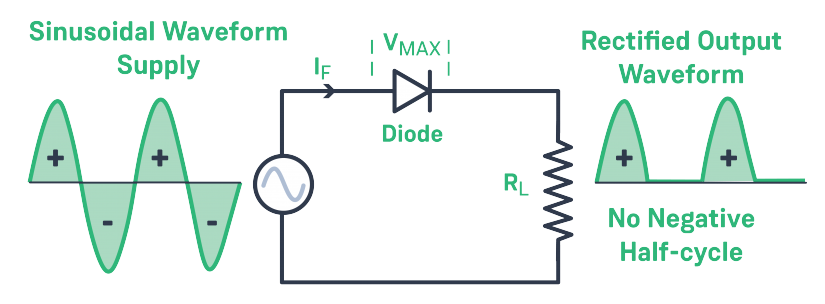
\includegraphics[width=0.75\linewidth]{img/rectifier.png}
    \caption{Half wave rectifier circuit}
    \label{fig:enter-label}
\end{figure}

\subsection*{Procedure:}
\begin{enumerate}
    \item \textbf{Circuit Construction:} Build the above given circuit on the breadboard:
    \begin{itemize}
        \item The half-wave bridge rectifier circuit is composed of a diode connected in series with a load resistor, $R_L$
        \item The input voltage and load resistor ($R_L$) are connected to the two channels of the oscilloscope to observe the waveforms.
    \end{itemize}

    \item \textbf{Setting Up the Signal Generator:}
    \begin{itemize}
        \item Set the signal generator to output a sinusoidal waveform (AC).
        \item Adjust the amplitude of the output signal to a suitable level (e.g., $5V$ peak-to-peak).
        \item Start with a low frequency (e.g., $50$ Hz).
    \end{itemize}

    \item \textbf{Observing the Waveform:}
    \begin{itemize}
        \item Connect the oscilloscope probes to the input and output (across the load resistor) of the circuit.
        \item Adjust the oscilloscope settings (vertical scale, horizontal scale, and trigger) to obtain a clear view of the waveforms.
    \end{itemize}

    \item \textbf{Analysis:}
    \begin{itemize}
        \item Sketch the input and output waveforms observed on the oscilloscope.
        \item Measure the peak-to-peak voltage of the output waveform.
        \item Verify that the output waveform is rectified (converted to a pulsating DC waveform).
    \end{itemize}
\end{enumerate}

\subsection*{Data and Calculations:}
\begin{itemize}
    \item Record the measured peak-to-peak voltage of the input and output waveforms.
    \item Calculate the average DC voltage at the output using a multimeter. The DC voltage at the output is given by

    $$  V_{dc} = \frac{V_P - V_b}{\pi} $$

    Where, $V_P$ = Peak input voltage and $V_b$ = built-in voltage ($0.7V$ for silicon diode)

    \item When a voltmeter measures the input voltage, the root-mean-square voltage must satisfy

    $$V_{rms} = \frac{V_P}{\sqrt{2}}$$
\end{itemize}

\subsection*{Observation Table:}

\begin{table}[h]
    \centering
    \begin{tabular}{c|m{1.5 cm}|m{1.5 cm}|m{2.75 cm}|c}
        \hline
        Resistance, $R_L$ & $V_{dc}$ & $V_{rms}$ & $I_{dc} = V_{dc} / R_L$ & $I_{rms} = V_{rms} / R_L$ \\ \hline
         &   &   &   &    \\ \hline
    \end{tabular}
    \label{tab:rectify}
\end{table}

\subsection*{Conclusion:}
By analyzing the waveforms and DC voltage measurement, verify the operation of the half wave rectifier circuit in converting AC voltage to pulsating DC voltage.

\newpage